\documentclass[11pt,a4paper]{article}

% ---- Encoding and fonts ----
\usepackage[T1]{fontenc}
\usepackage[utf8]{inputenc}
\usepackage{lmodern}
\usepackage{microtype}

% ---- Page geometry and spacing ----
\usepackage[a4paper,margin=2.5cm]{geometry}
\usepackage{setspace}
\onehalfspacing

% ---- Mathematics ----
\usepackage{amsmath,amssymb,amsthm,mathtools}
\numberwithin{equation}{section}

% ---- Graphics, diagrams, tables, captions ----
\usepackage{graphicx}
\usepackage{float}
\graphicspath{{../results/figures/}}
\usepackage{tikz}
\usetikzlibrary{arrows.meta,positioning,calc}
\usepackage{booktabs}
\usepackage{caption}
\captionsetup{font=small,labelfont=bf}

% ---- Links and cross-references ----
\usepackage{xcolor}
\definecolor{linknavy}{RGB}{0,51,102}
\usepackage[colorlinks=true,linkcolor=linknavy,citecolor=linknavy,urlcolor=linknavy]{hyperref}
\usepackage{cleveref}

% ---- Theorem environments ----
\theoremstyle{definition}
\newtheorem{definition}{Definition}[section]
\theoremstyle{plain}
\newtheorem{proposition}{Proposition}[section]
\theoremstyle{remark}
\newtheorem{remark}{Remark}[section]

% ---- Convenience macros ----
\newcommand{\E}{\mathbb{E}}
\newcommand{\Q}{\mathbb{Q}}
\newcommand{\PP}{\mathbb{P}}
\newcommand{\R}{\mathbb{R}}
\newcommand{\dd}{\,\mathrm{d}}
\DeclareMathOperator{\Var}{Var}

\title{\bfseries Numerical Methods for Option Pricing\\[0.3em]
  \large Stability, Convergence and Early Exercise}
\author{Benjamin Mellors\\[0.3em]
  \normalsize Independent project\\
  \normalsize University of Surrey}
\date{June 2026}

\begin{document}

% ---- Title page ----
\begin{titlepage}
  \centering
  \vspace*{\fill}
  {\Huge\bfseries Numerical Methods for Option Pricing\par}
  \vspace{0.9em}
  {\Large Stability, Convergence and Early Exercise\par}
  \vspace{2.8em}
  \rule{0.55\textwidth}{0.4pt}\par
  \vspace{2.8em}
  {\large Benjamin Mellors\par}
  \vspace{0.7em}
  {\normalsize Independent project\par}
  {\normalsize University of Surrey\par}
  \vspace{2.8em}
  {\normalsize June 2026\par}
  \vspace*{\fill}
\end{titlepage}

% ---- Front matter (roman numerals) ----
\pagenumbering{roman}

\begin{abstract}
\noindent
This report prices European call and put options by four methods: the
closed-form Black--Scholes formula, a Cox--Ross--Rubinstein binomial tree, Monte
Carlo simulation, and an explicit finite-difference solver for the Black--Scholes
equation, and extends the binomial method to American options. The four methods
agree on a benchmark price to within the expected numerical error, which fixes
the implementation. The closed-form price, being exact, then serves as a
yardstick for studying the schemes: the binomial tree's oscillatory convergence,
Monte Carlo's slow $1/\sqrt{n}$ error decay, and, for the finite-difference
method, the conditional stability of the explicit scheme together with its
second-order convergence in the space step. The American extension introduces
the early-exercise decision, an optimal stopping problem with no closed-form
solution, handled in the tree by a single comparison at each node.
\end{abstract}

\newpage
\tableofcontents

\newpage
\pagenumbering{arabic}

% =====================================================================
\section{Introduction}\label{sec:intro}

An option is a contract whose value depends on the uncertain future price of an
underlying asset. Pricing it means assigning a fair value today, before that
price is known. For the simplest contract under the simplest model, a European
option on a stock following geometric Brownian motion, there is an exact answer,
the Black--Scholes formula. Most contracts of practical interest have no such
closed form and must be priced numerically.

This report takes the problem that \emph{does} have an exact answer and prices it
four different ways: the Black--Scholes formula itself, a binomial tree, Monte
Carlo simulation, and a finite-difference solver for the Black--Scholes partial
differential equation. Because the exact price is known, each numerical method
can be checked against it, and its characteristic behaviour, how quickly it
converges and when it breaks down, can be studied in a setting where the right
answer is not in doubt. The same methods carry over to problems with no closed
form; the controlled study here is what justifies trusting them there. The
binomial method is then extended to American options, which can be exercised
early and so have no closed-form price even under this model.

The scope is deliberately narrow. The underlying follows geometric Brownian
motion with constant volatility and a constant risk-free rate, and the contracts
are vanilla European and American calls and puts. The point is not to model
market frictions but to study the numerical methods themselves against a known
answer.

This project was completed independently during the second year of a BSc in
Financial Mathematics at the University of Surrey, drawing in places on
material beyond what has been formally covered in the degree at this point.
Results that depend on that material, such as the derivation of the
Black--Scholes equation itself, are cited to the standard references rather
than re-derived; the contribution here is the implementation, cross-validation
and numerical analysis of the four methods.

\Cref{sec:model} sets up the model and the risk-neutral pricing rule that every
method uses. \Cref{sec:analytic} gives the Black--Scholes formula, which is the
benchmark. \Cref{sec:binomial,sec:montecarlo,sec:pde} develop the three numerical
methods in turn, the last of these, the finite-difference scheme, being where
stability and convergence are studied most closely. \Cref{sec:american} treats
American options and early exercise, and \Cref{sec:conclusion} draws the methods
together and notes what each leaves for further work. All results are produced by
a tested implementation and are reproducible.

% =====================================================================
\clearpage
\section{The model and risk-neutral valuation}\label{sec:model}

Every method in this report prices the same object, a European option on a
single stock, and rests on the same two ingredients: a model for how the stock
moves, and a rule for turning that model into a price. This section sets out
both. The model is geometric Brownian motion; the pricing rule is risk-neutral
valuation, which follows from the absence of arbitrage. The argument that
produces the pricing rule also produces the Black--Scholes partial differential
equation, which the finite-difference method later solves directly.

\subsection{The underlying asset}

We model the stock price $S_t$ as geometric Brownian motion,
\begin{equation}\label{eq:gbm}
  \dd S_t = \mu S_t \dd t + \sigma S_t \dd W_t.
\end{equation}
The equation has two parts. The first, $\mu S_t \dd t$, is the \emph{drift}: a
steady trend, with $\mu$ the stock's expected rate of return. The second,
$\sigma S_t \dd W_t$, is the \emph{shock}: a random fluctuation, with
$\sigma > 0$ the volatility and $W_t$ Brownian motion.

Both terms are scaled by $S_t$, for two reasons. First, it expresses a move as
a proportion of the current price rather than a fixed number of pounds: a £1
change matters far more to a £10 stock than to a £100 stock, so scaling by
$S_t$ puts moves of different stocks, or of the same stock at different price
levels, on a comparable footing. Second, it keeps the price positive: the
model only ever multiplies $S_t$ by something, never subtracts a fixed amount
that could push it below zero, which a share price cannot do.

The random term $\dd W_t$ is built from Brownian motion. Over a small time
step $\dd t$ it can be written
\[
  \dd W_t = \varepsilon \sqrt{\dd t}, \qquad \varepsilon \sim N(0,1),
\]
a standard normal draw scaled by $\sqrt{\dd t}$. The square-root scaling
reflects how randomness accumulates: shocks over non-overlapping time
intervals are independent, and variance adds across independent quantities, so
the variance built up after a time $t$ is proportional to $t$, and the
standard deviation, the typical size of the accumulated move, is
proportional to $\sqrt{t}$.

$\sigma$ is quoted on an annual basis. Informally, under this model around two
years out of three see an annual return within one standard deviation of its
average, so $\sigma = 20\%$ corresponds to yearly moves of roughly $\pm 20\%$
being unremarkable rather than extreme.

\subsection{The pricing problem}

A European option is a contract paying a fixed function of $S_T$ at a maturity
$T$, and nothing before. A call with strike $K$ pays
\[
  (S_T - K)^{+} = \max(S_T - K,\, 0),
\]
and a put pays $(K - S_T)^{+}$. The task is to value the contract at $t = 0$.

The obvious guess, discounting the expected payoff using your own forecast of
the stock's chances, fails. It depends on $\mu$, the stock's expected return,
which different investors estimate differently; a price all of them can agree
on cannot depend on it. The resolution, set out next, is to discount using a
different, agreed set of odds instead of anyone's personal forecast.

\subsection{Risk-neutral valuation}

Write $V(S,t)$ for the value of the option at a future time $t$ if the stock
is at level $S$ then. In particular $V(S_0, 0)$ is today's price, with $S_0$
today's stock price: the quantity this report is ultimately after.

The stock's expected return $\mu$ and the risk-free rate $r$ are different
numbers. $\mu$ is the average return of the stock itself, a risky asset; $r$
is the safe return available from something like a government bond. $\mu$ is
normally higher than $r$, because investors need some extra reward for
holding a risky asset rather than a safe one. Pricing the option using $\mu$
would mean pricing it using how large a reward each investor personally
demands for that risk, which is not something everyone agrees on.

The standard fix is to price the option exactly as before, a discounted
average payoff, but with $\mu$ replaced by $r$ throughout the calculation:
\begin{equation}\label{eq:rn-price}
  V(S_0, 0) = e^{-rT}\,\overline{\mathrm{payoff}(S_T)},
\end{equation}
where the bar denotes the average payoff, computed assuming the stock grows
at rate $r$ rather than $\mu$. That this substitution gives the correct price
is a standard no-arbitrage result, established in the original Black--Scholes
paper \cite{blackscholes}. It is stated here rather than derived,
because the result itself is what the report uses: with $\mu$ replaced by
$r$, the price no longer depends on anyone's personal view of the stock.
\Cref{sec:binomial} carries out exactly this substitution by hand, for a
single up-or-down step.

Under this substitution, the terminal stock price follows the same kind of
formula as before with $\mu$ replaced by $r$,
\begin{equation}\label{eq:terminal}
  S_T = S_0 \exp\!\left( \left(r - \tfrac{1}{2}\sigma^2\right)T
        + \sigma\sqrt{T}\,Z \right), \qquad Z \sim N(0,1).
\end{equation}
This is the law sampled directly by the Monte Carlo method (\cref{sec:montecarlo})
and integrated in closed form by the Black--Scholes formula (\cref{sec:analytic}).

\subsection{The Black--Scholes equation}

Equation~\eqref{eq:rn-price} has an equivalent description as a partial
differential equation. Under the same model, the price $V(S,t)$ can be shown
to satisfy the Black--Scholes equation,
\begin{equation}\label{eq:bspde}
  \frac{\partial V}{\partial t}
  + \tfrac{1}{2}\sigma^2 S^2 \frac{\partial^2 V}{\partial S^2}
  + r S \frac{\partial V}{\partial S} - rV = 0,
\end{equation}
to be solved backwards from the payoff specified at $t = T$. This equation is
derived in the original Black--Scholes paper \cite{blackscholes}; it is stated
here because \cref{sec:pde} solves it directly
by finite differences. As with \eqref{eq:rn-price}, $\mu$ does not appear:
both describe the same risk-neutral price, one as an expectation and the other
as a PDE, depending only on $S$, $r$ and $\sigma$.

% =====================================================================
\clearpage
\section{The Black--Scholes formula}\label{sec:analytic}

For a European call or put, the expectation \eqref{eq:rn-price} over the
lognormal terminal law \eqref{eq:terminal} evaluates in closed form to the
Black--Scholes formula \cite{blackscholes}. For strike $K$ and maturity
$T$,
\begin{align}
  C &= S\,\Phi(d_1) - K e^{-rT}\Phi(d_2), \label{eq:bscall}\\
  P &= K e^{-rT}\Phi(-d_2) - S\,\Phi(-d_1), \label{eq:bsput}
\end{align}
where $\Phi$ is the standard normal distribution function and
\begin{equation}\label{eq:d1d2}
  d_1 = \frac{\ln(S/K) + \left(r + \tfrac{1}{2}\sigma^2\right)T}{\sigma\sqrt{T}},
  \qquad
  d_2 = d_1 - \sigma\sqrt{T}.
\end{equation}

The two terms of the call \eqref{eq:bscall} have a direct reading. The second,
$K e^{-rT}\Phi(d_2)$, is the strike, discounted to present value because it is
paid at $T$, and weighted by $\Phi(d_2)$, the risk-neutral probability of
exercise. The holder pays $K$ only in the states where exercise
happens, which is why the strike enters discounted and probability-weighted
rather than as $K$. The first term is the corresponding present value of
receiving the stock in those states.

The quantities $d_1$ and $d_2$ are not arbitrary. From
\cref{sec:model}, the terminal price satisfies
$\ln(S_T/S) \sim N\!\big((r-\tfrac{1}{2}\sigma^2)T,\ \sigma^2 T\big)$. The call
finishes in the money when $S_T > K$, equivalently $\ln(S_T/S) > \ln(K/S)$;
standardising this event against the known mean and
standard deviation of $\ln(S_T/S)$ gives exactly $d_2$, so $d_2$ measures, in
standard deviations, how far today's price sits above the strike once the
risk-neutral drift is accounted for, and $\Phi(d_2)$ is the
probability of that event. At the benchmark parameters $d_2 = 0.15$ and
$\Phi(d_2) \approx 0.56$, a fractionally better than even chance the call
finishes in the money. The other quantity,
$d_1 = d_2 + \sigma\sqrt{T}$, is $d_2$ shifted by one unit of
volatility, which weights the first term $S\,\Phi(d_1)$ correctly as the
present value of the stock received on exercise. Unlike $\Phi(d_2)$,
$\Phi(d_1)$ is not an ordinary probability: it is a truncated expectation,
averaging $S_T$ only over the scenarios where the option finishes in the
money, so it already has how far above $K$ baked in, as well as how likely. It
also has a more concrete identity: $\Phi(d_1)$ is the option's
delta, $\partial C/\partial S$, the amount the price moves for a
£1 move in the stock. The reason for the shift between $d_1$ and
$d_2$ involves a change of probability measure, a standard result of the
risk-neutral pricing theory that is beyond this report's scope. At the
benchmark parameters $d_1 = 0.35$ and
$\Phi(d_1) \approx 0.64$.

A relation that does not depend on the model links the two. Subtracting
\eqref{eq:bsput} from \eqref{eq:bscall},
\begin{equation}\label{eq:parity}
  C - P = S - K e^{-rT}.
\end{equation}
This is put--call parity, and it follows from the payoffs alone by a no-arbitrage
argument: a portfolio long a call and short a put has the same payoff at $T$ as
holding the stock and borrowing $K e^{-rT}$, so the two must cost the same today.
It holds whatever prices a model assigns, so is a clean check on any pricer.

At the benchmark parameters used throughout ($S = K = 100$, $r = 5\%$,
$\sigma = 20\%$, $T = 1$), formula \eqref{eq:bscall} gives a call price of
$10.4506$. The implementation reproduces this, and put--call parity
\eqref{eq:parity} holds to machine precision, both checked in the test suite:
the reference for the three methods below.

% =====================================================================
\section{The binomial tree}\label{sec:binomial}

The binomial method replaces continuous time with a finite number of steps. Over
each step the stock makes one of two moves, and the option is priced by working
backwards from its payoff. As the number of steps grows, the price converges to
the Black--Scholes value.

\subsection{Construction}

Divide $[0,T]$ into $N$ steps of length $\Delta t = T/N$. Over one step the price
either multiplies by $u > 1$ or by $d < 1$. The Cox--Ross--Rubinstein choice
\cite{crr} sets
\begin{equation}\label{eq:crr-ud}
  u = e^{\sigma\sqrt{\Delta t}}, \qquad d = e^{-\sigma\sqrt{\Delta t}} = \frac{1}{u},
\end{equation}
which makes the tree recombine: an up move followed by a down move returns to
the starting price, so that after $n$ steps there are only $n+1$ distinct prices
rather than $2^n$. The step is priced under the risk-neutral measure of
\cref{sec:model}: requiring the expected one-step growth to equal the risk-free
rate, $p\,u + (1-p)\,d = e^{r\Delta t}$, fixes the risk-neutral probability of an
up move. Expanding the constraint, $p\,u + d - p\,d = e^{r\Delta t}$, so
$p\,(u-d) = e^{r\Delta t} - d$, and dividing through by $(u-d)$ gives
\begin{equation}\label{eq:crr-p}
  p = \frac{e^{r\Delta t} - d}{u - d}.
\end{equation}
Read as a probability, $p$ is the chance of an up move and $1-p$ the chance of
a down move; the two automatically sum to one, since $1-p$ simplifies to
$(u - e^{r\Delta t})/(u-d)$, the same fraction with the numerator's two terms
swapped. This $p$ is the same kind of substitution introduced in
\cref{sec:model}: it
is not a forecast of which way the stock will actually move, but the value
that makes the stock's expected one-step growth match the risk-free rate $r$,
in place of the stock's real drift.
\Cref{fig:tree} shows the first few steps.

\begin{figure}[H]
  \centering
  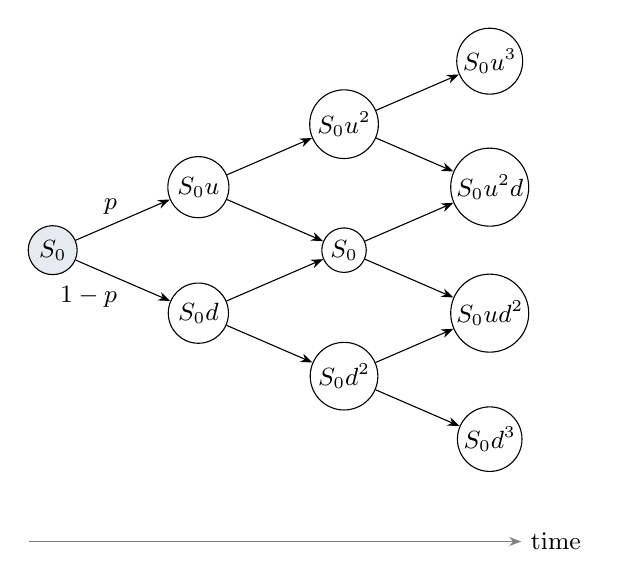
\begin{tikzpicture}[>={Stealth[scale=0.9]},every node/.style={font=\small}]
    \def\dx{1.85}\def\dy{0.8}
    \node[circle,draw,fill=linknavy!10,inner sep=2pt] (n00) at (0,0) {$S_0$};
    \node[circle,draw,inner sep=2pt] (n11) at (\dx,\dy) {$S_0u$};
    \node[circle,draw,inner sep=2pt] (n10) at (\dx,-\dy) {$S_0d$};
    \node[circle,draw,inner sep=1.4pt] (n22) at (2*\dx,2*\dy) {$S_0u^2$};
    \node[circle,draw,inner sep=1.4pt] (n21) at (2*\dx,0) {$S_0$};
    \node[circle,draw,inner sep=1.4pt] (n20) at (2*\dx,-2*\dy) {$S_0d^2$};
    \node[circle,draw,inner sep=1pt] (n33) at (3*\dx,3*\dy) {$S_0u^3$};
    \node[circle,draw,inner sep=1pt] (n32) at (3*\dx,\dy) {$S_0u^2d$};
    \node[circle,draw,inner sep=1pt] (n31) at (3*\dx,-\dy) {$S_0ud^2$};
    \node[circle,draw,inner sep=1pt] (n30) at (3*\dx,-3*\dy) {$S_0d^3$};
    \draw[->] (n00)--(n11) node[midway,above left=-2pt]{$p$};
    \draw[->] (n00)--(n10) node[midway,below left=-2pt]{$1-p$};
    \draw[->] (n11)--(n22); \draw[->] (n11)--(n21);
    \draw[->] (n10)--(n21); \draw[->] (n10)--(n20);
    \draw[->] (n22)--(n33); \draw[->] (n22)--(n32);
    \draw[->] (n21)--(n32); \draw[->] (n21)--(n31);
    \draw[->] (n20)--(n31); \draw[->] (n20)--(n30);
    \draw[->,gray] (-0.3,-3.7) -- (3*\dx+0.4,-3.7) node[right,black]{time};
  \end{tikzpicture}
  \caption{The first three steps of a recombining CRR tree. Each step moves up by
    a factor $u$ with risk-neutral probability $p$ or down by $d$ with
    probability $1-p$; an up move and a down move recombine to the same price.}
  \label{fig:tree}
\end{figure}

\subsection{Pricing by backward induction}

At maturity the value at each terminal node is just the payoff. Stepping back one
level, a node's value is the discounted risk-neutral expectation of the two nodes
it leads to,
\begin{equation}\label{eq:crr-back}
  V = e^{-r\Delta t}\big[\,p\,V_{\text{up}} + (1-p)\,V_{\text{down}}\,\big],
\end{equation}
which is \eqref{eq:rn-price} applied over a single step. Repeating \eqref{eq:crr-back}
from the terminal layer back to the root gives the price today.

\subsection{Convergence}

As $N \to \infty$ the tree price converges to the Black--Scholes value, but not
smoothly: it does not approach $10.4506$ steadily from one side. \Cref{fig:conv-binomial}
plots the price against $N$, and it wobbles, landing alternately a little too
high and a little too low as $N$ increases by one each time, with the wobble
shrinking as $N$ grows. To be precise about what is wobbling: each value of
$N$ defines one tree, and that whole tree collapses by backward induction to a
single number, the price. It is this single number, one per $N$, that is
plotted against $N$, not the scatter of terminal prices inside any one tree.

\Cref{tab:terminal-nodes} makes the link between the two concrete, for $N=2$
and $N=3$ at the benchmark parameters ($S_0 = K = 100$, $\sigma = 20\%$,
$T = 1$). The payoff $\max(S-K,0)$ has a kink at $S = K$: it is flat below $K$
and rises linearly above it. With $N = 2$, one of the three terminal prices
lands exactly on $K$, because a recombining tree always has a path with
equally many up and down moves when $N$ is even, and an equal number of up and
down moves returns the price to its starting level. With $N = 3$, no terminal
price is anywhere near $K$, because an odd number of steps cannot be split
into two equal halves; the nearest prices sit more than £11 away on either
side.

\begin{table}[H]
  \centering
  \begin{tabular}{lccc}
    \toprule
    & Terminal prices & Closest to $K = 100$ & Resulting price \\
    \midrule
    $N = 2$ (even) & $75.4,\ \mathbf{100.0},\ 132.7$ & $100.0$, exact &
      $9.54$ \ (£0.91 below) \\
    $N = 3$ (odd)  & $70.7,\ 89.1,\ 112.2,\ 141.4$ & over £11 away &
      $11.04$ \ (£0.59 above) \\
    \bottomrule
  \end{tabular}
  \caption{Terminal tree prices for $N = 2$ and $N = 3$ at $S_0 = K = 100$,
    and the single price each whole tree produces. These are the first two
    points plotted in \cref{fig:conv-binomial}.}
  \label{tab:terminal-nodes}
\end{table}

The last column is the payoff for understanding the wobble: $N=2$, with a node
sitting exactly on the kink, undershoots the true price by £0.91; $N=3$, with
a gap straddling the kink, overshoots it by £0.59. A node on the kink
lets that tree price the region around $K$ more accurately than a tree with
only a gap there, and this difference in accuracy is what pushes the computed
price to one side of the true value or the other. The pattern holds generally:
every even $N$ undershoots, every odd $N$ overshoots, and both gaps shrink
steadily as $N$ grows, the decaying zig-zag visible in \cref{fig:conv-binomial}.
The precise size of the under- and over-shoot at each $N$ follows formally
from how a discrete sum approximates a kinked function, treated in the original
CRR paper \cite{crr}; node position relative to $K$ is
the mechanism demonstrated here.

\begin{figure}[H]
  \centering
  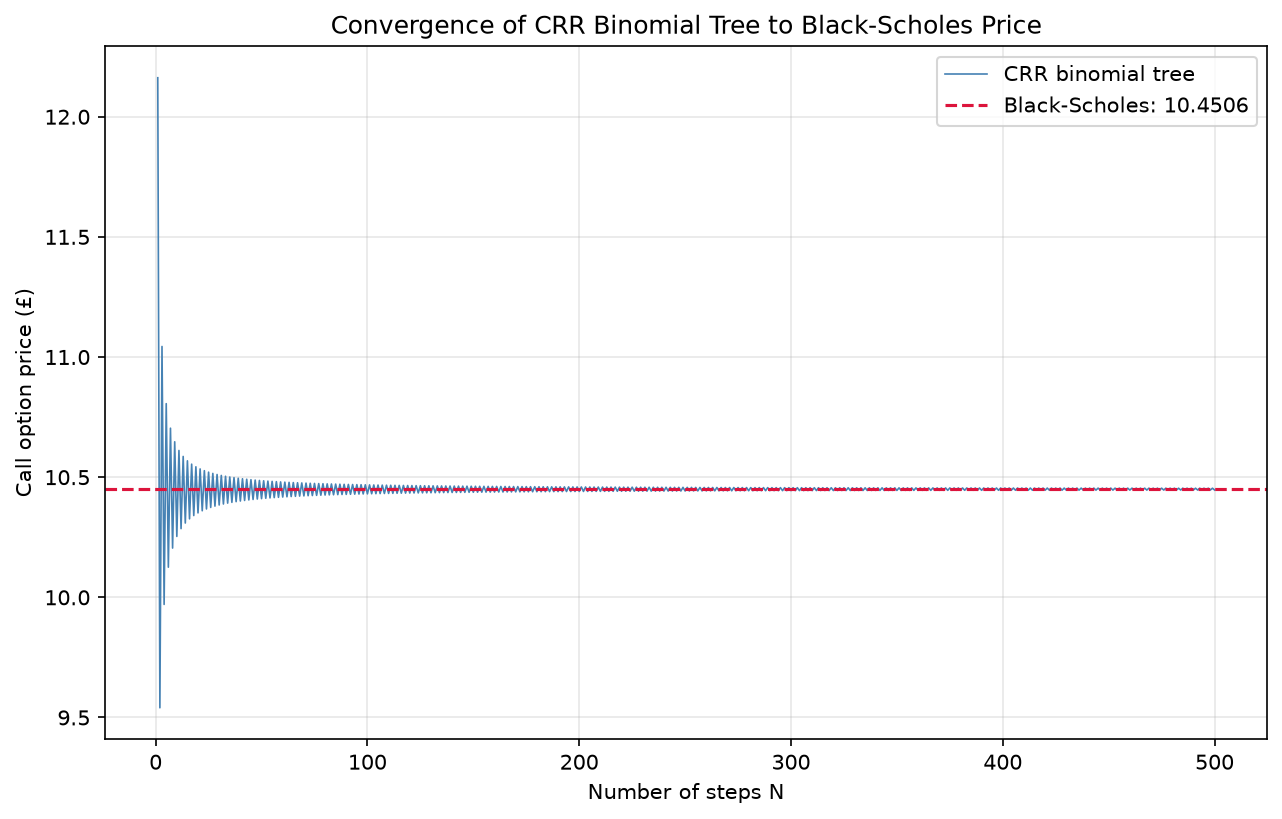
\includegraphics[width=0.92\textwidth]{convergence_binomial.png}
  \caption{Binomial price against the number of steps $N$. The price converges to
    the Black--Scholes value with the characteristic odd--even oscillation, which
    decays as the step count grows.}
  \label{fig:conv-binomial}
\end{figure}

At $N = 5000$ the tree gives $10.4502$, matching the Black--Scholes price to three
decimal places; the test suite checks agreement at large $N$. The method
demonstrates a fully discrete scheme converging to the continuous-time price, with
the oscillation a visible feature of how the discrete and continuous problems
relate.

% =====================================================================
\clearpage
\section{Monte Carlo simulation}\label{sec:montecarlo}

Monte Carlo prices the option through the expectation form \eqref{eq:rn-price}
directly: it estimates the discounted expected payoff by averaging over simulated
outcomes.

\subsection{The estimator}

For a European payoff only the terminal price $S_T$ matters, so it can be sampled
directly from the lognormal law \eqref{eq:terminal} without simulating the path in
between. Drawing $n$ independent standard normals $Z_1,\dots,Z_n$ and setting
$S_T^{(j)} = S_0 \exp\!\big((r-\tfrac{1}{2}\sigma^2)T + \sigma\sqrt{T}\,Z_j\big)$ -
the bracketed superscript $(j)$ labels the $j$-th simulated price, not a power -
the price is estimated by the discounted sample mean of the payoffs,
\begin{equation}\label{eq:mc-est}
  \widehat{V}_n = e^{-rT}\,\frac{1}{n}\sum_{j=1}^{n} \big(S_T^{(j)} - K\big)^{+}.
\end{equation}
The estimator is unbiased: averaged over many repetitions, it returns exactly
the Black--Scholes price.

\subsection{Error and convergence}

In plain terms: run the simulation once and the estimator returns one number;
run it again with a fresh batch of random draws and it returns a slightly
different number. The standard error measures how much these estimates
typically vary from one batch to the next, and how that variation shrinks as
more paths are simulated.

More precisely, by the central limit theorem $\widehat{V}_n$ is approximately
normal about the
true price with standard deviation $s/\sqrt{n}$, where $s$ is the sample standard
deviation of the discounted payoffs. This standard error sets the size of the
estimate's likely error, and it shrinks only as $1/\sqrt{n}$. Because the $n$
sits under a square root, halving the error needs $\sqrt{n}$ to double, which
needs $n$ itself to be multiplied by four: $\sqrt{4n} = 2\sqrt{n}$. The slow
rate is the method's defining limitation,
and the price of its generality: the same estimator works in any number of
dimensions and for any payoff, where the lattice and the PDE become expensive or
intractable. The simulation uses a fixed random seed, so every reported figure
is reproducible.

\Cref{fig:conv-mc} shows the estimate settling onto the Black--Scholes price as
$n$ grows, with the swings around the limit shrinking as the standard error
falls at the $1/\sqrt{n}$ rate. At
$n = 10^{6}$ paths, the $n$ discounted payoffs have a sample standard deviation
of $s \approx 14.73$; dividing by $\sqrt{n} = 1000$ gives the standard error
quoted earlier, $s/\sqrt{n} = 14.73/1000 = 0.0147$, so the estimate is
$10.4532 \pm 0.0147$. This is consistent with the exact price $10.4506$, lying
within about two standard errors of it. The test suite checks that the
estimate falls within a set tolerance of the Black--Scholes value.

\begin{figure}[H]
  \centering
  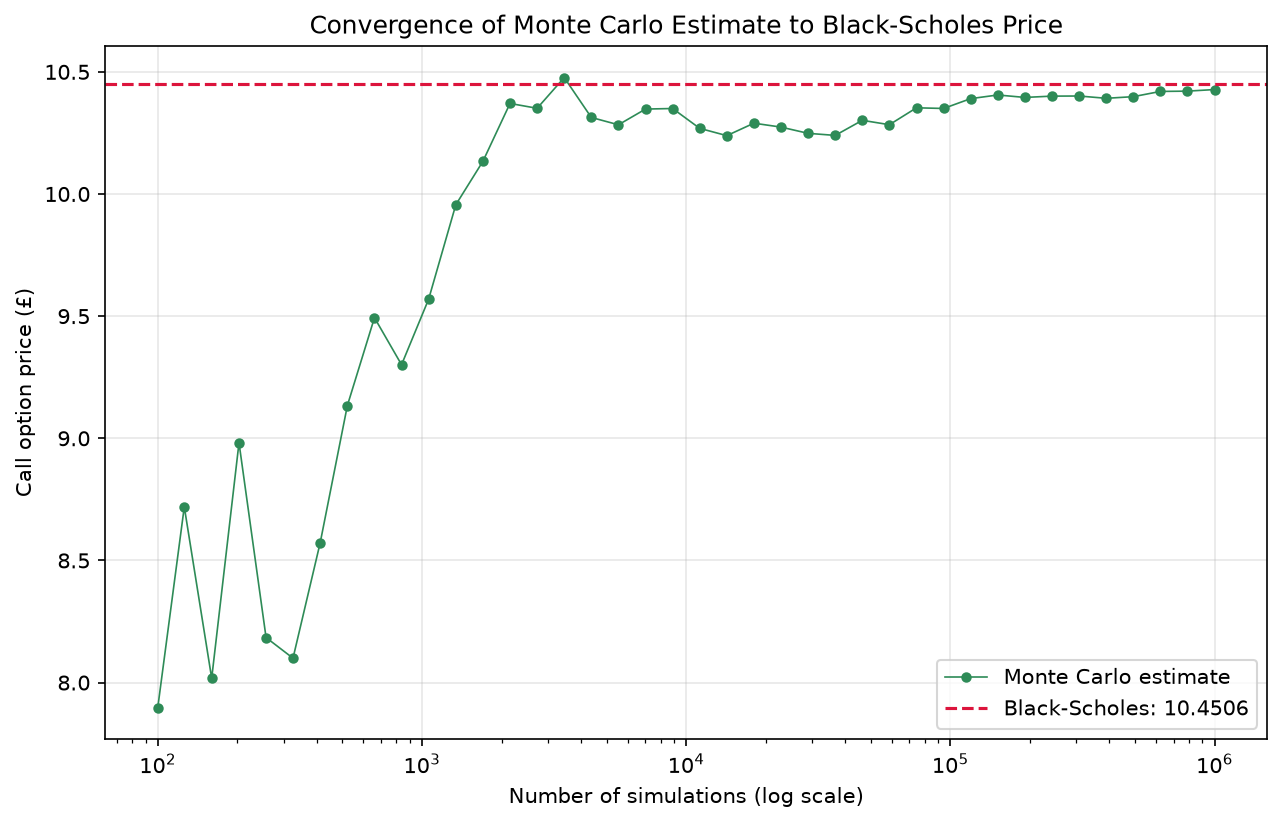
\includegraphics[width=0.92\textwidth]{convergence_montecarlo.png}
  \caption{Monte Carlo price against the number of simulated paths $n$. The
    estimate settles onto the Black--Scholes price as
    the standard error shrinks at the $1/\sqrt{n}$ rate.}
  \label{fig:conv-mc}
\end{figure}

The method demonstrates an unbiased probabilistic estimator whose error is
controlled by sample size rather than by a step length, converging slowly but in
a way that does not depend on dimension.

% =====================================================================
\clearpage
\section{The finite-difference method}\label{sec:pde}

The finite-difference method solves the Black--Scholes equation \eqref{eq:bspde}
directly, by replacing the derivatives with differences on a grid and marching
backwards from the payoff. It is the method that generalises most readily to
problems with no closed form, and it is also the one whose numerical behaviour,
stability and convergence, most repays study, because both can be made precise
and then checked against the exact price; a standard treatment of finite-difference
schemes for parabolic equations of this kind is given in Ammari \cite{ammari}.

The scheme developed here is called \emph{explicit} because each new value is
computed directly from values that are already known, with no equations left
to solve. The alternative, an \emph{implicit} scheme, writes the new time
level in terms of \emph{other unknown} values at that same new time level, so
every step requires solving a system of equations simultaneously rather than
just substituting numbers in. Implicit schemes cost more per step for exactly
that reason, but, as noted in \cref{sec:conclusion}, they buy unconditional
stability in return; the explicit scheme here is simpler to implement and to
reason about, at the cost of the stability condition derived below.

\subsection{Discretisation}

Lay down a grid with prices $S_i = i\,\Delta S$ for $i = 0,\dots,M$ and times
$t_n = n\,\Delta t$ for $n = 0,\dots,N$, and write $V_i^{\,n}$ for the
approximation to $V(S_i,t_n)$. The terminal condition fixes $V_i^{\,N}$ as the
payoff, and the boundary conditions at $S=0$ and $S = S_M$ are known; the scheme
fills in the interior by marching backwards in time.

The \emph{explicit} scheme replaces every derivative in \eqref{eq:bspde} with a
difference between neighbouring grid values: each first derivative becomes a
difference across adjacent nodes, and the second derivative a difference of
those differences. Substituting these into \eqref{eq:bspde} and rearranging
for $V_i^{\,n}$ gives the update rule used in the implementation, in which each
value at one time level is a weighted combination of three values at the next:
\begin{equation}\label{eq:fd-update}
  V_i^{\,n} = a_i\,V_{i-1}^{\,n+1} + b_i\,V_i^{\,n+1} + c_i\,V_{i+1}^{\,n+1},
\end{equation}
with coefficients
\begin{equation}\label{eq:fd-coeffs}
  a_i = \tfrac{1}{2}\Delta t\,(\sigma^2 i^2 - r i), \qquad
  b_i = 1 - \Delta t\,(\sigma^2 i^2 + r), \qquad
  c_i = \tfrac{1}{2}\Delta t\,(\sigma^2 i^2 + r i).
\end{equation}
Here $i$ is the price-step index, so $S_i = i\,\Delta S$. Each interior value at
one time level is built from three values at the next, as
in the stencil of \cref{fig:stencil}.

\begin{figure}[H]
  \centering
  \begin{tikzpicture}[>={Stealth[scale=0.9]},every node/.style={font=\small}]
    \def\g{1.15}
    \foreach \n in {0,...,5}{ \foreach \i in {0,...,4}{
      \fill[black!22] (\n*\g,\i*\g) circle (1.4pt); }}
    \coordinate (tgt) at (1*\g,2*\g);
    \coordinate (sD) at (2*\g,1*\g);
    \coordinate (sM) at (2*\g,2*\g);
    \coordinate (sU) at (2*\g,3*\g);
    \draw[->,linknavy,thick] (sD)--(tgt);
    \draw[->,linknavy,thick] (sM)--(tgt);
    \draw[->,linknavy,thick] (sU)--(tgt);
    \fill[linknavy] (sD) circle (2.5pt); \fill[linknavy] (sM) circle (2.5pt);
    \fill[linknavy] (sU) circle (2.5pt);
    \fill[red!80!black] (tgt) circle (2.5pt);
    \node[red!80!black,below=2pt] at (tgt) {$V_i^{\,n}$};
    \node[linknavy,right=3pt] at (sM) {$V_i^{\,n+1}$};
    \node[linknavy,right=3pt] at (sU) {$V_{i+1}^{\,n+1}$};
    \node[linknavy,right=3pt] at (sD) {$V_{i-1}^{\,n+1}$};
    \draw[->] (-0.3,0) -- (5*\g+0.6,0) node[right]{$t$\;(index $n$)};
    \draw[->] (0,-0.3) -- (0,4*\g+0.5) node[above]{$S$\;(index $i$)};
    \draw[<->] (0,-0.55) -- (\g,-0.55) node[midway,below]{$\Delta t$};
    \draw[<->] (-0.55,0) -- (-0.55,\g) node[midway,left]{$\Delta S$};
  \end{tikzpicture}
  \caption{The explicit stencil. The value at an interior node $(i,n)$ is a
    weighted combination of three nodes at the next time level, $(i-1,n+1)$,
    $(i,n+1)$ and $(i+1,n+1)$, with weights $a_i$, $b_i$ and $c_i$ from
    \eqref{eq:fd-coeffs}. The scheme marches backwards in time from the payoff.}
  \label{fig:stencil}
\end{figure}

\subsection{Stability}

The update \eqref{eq:fd-update} is a weighted combination of three values. If the
weights are non-negative the combination is \emph{monotone}: it behaves like a
weighted average, and a weighted average can never fall outside the range of
its ingredients, the way a mixture of three jugs of water can never end up
colder than the coldest jug or hotter than the hottest. An error in the inputs
is therefore blended, not magnified, and the scheme is stable. The off-diagonal
weights $a_i$ and $c_i$ are non-negative for the relevant range of $i$, but the
central weight
\[
  b_i = 1 - \Delta t\,(\sigma^2 i^2 + r)
\]
can turn negative. This is the weight on $V_i^{\,n+1}$, the node directly to
the right of the target node in \cref{fig:stencil}, one time step ahead. Reading the formula, $b_i$ shrinks as
$i$ grows, because $\sigma^2 i^2$ grows with it, and shrinks further as
$\Delta t$ grows; once $\Delta t\,(\sigma^2 i^2 + r)$ exceeds $1$, $b_i$ flips
negative. At that point the scheme is no longer a weighted average: it has to
subtract a fraction of $V_i^{\,n+1}$ rather than add one, so the monotone
property above breaks, and the scheme becomes unstable. The binding case is
the largest index $i = M$, where the coefficient $\sigma^2 i^2$ is greatest;
requiring $b_M \ge 0$ gives $\Delta t \le 1/(\sigma^2 M^2 + r)$, or, with
$\Delta t = T/N$ and neglecting the small $r$ term,
\begin{equation}\label{eq:cfl}
  N \gtrsim \sigma^2 M^2 T.
\end{equation}
Below this threshold $b_M$ is negative, the scheme amplifies the
highest-frequency components of the error at every step, and the solution
diverges. (The same conclusion follows from von Neumann analysis, which tracks
the growth of Fourier modes under the scheme; the positivity argument here is its
elementary counterpart.)

\Cref{fig:pde-stability} shows both regimes at $M = 200$, where
\eqref{eq:cfl} requires $N \gtrsim \sigma^2 M^2 T = 1600$. With $N = 100$, far
below the threshold, the scheme is unstable: the solution reaches a magnitude
of around $10^{138}$ within a hundred time steps. With $N = 2000$, above the
threshold, it is well behaved and returns a price of $10.4550$.

\begin{figure}[H]
  \centering
  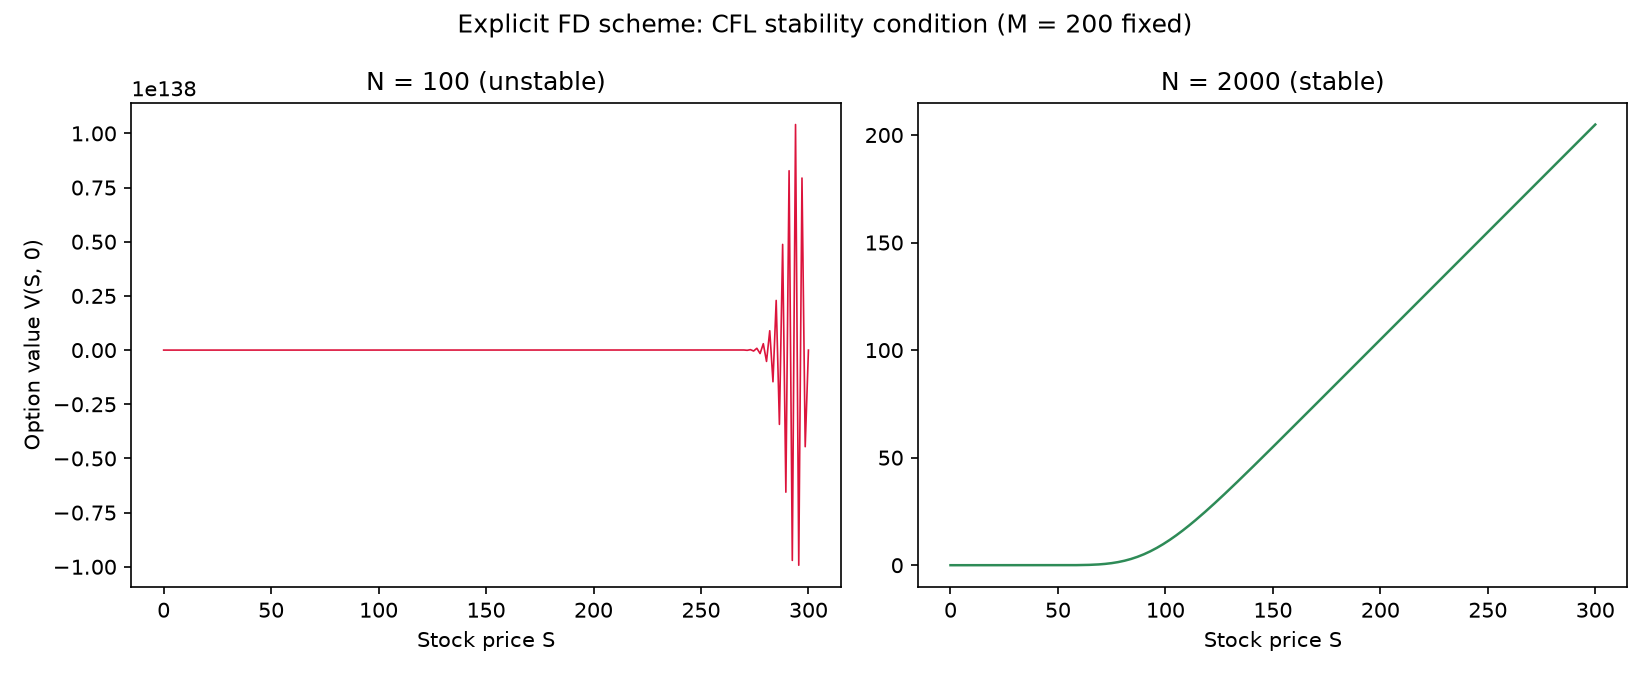
\includegraphics[width=0.98\textwidth]{pde_stability.png}
  \caption{The explicit scheme at fixed $M = 200$ under an unstable and a stable
    choice of time step. With $N = 100$ the stability condition \eqref{eq:cfl} is
    violated and the solution diverges (left); with $N = 2000$ it is satisfied and
    the scheme recovers the payoff structure and a correct price (right).}
  \label{fig:pde-stability}
\end{figure}

\subsection{Convergence}

With stability ensured, the question is how quickly the price approaches the
exact answer as the grid is refined. The difference formulas used in
\cref{sec:pde} only approximate the true derivatives they stand in for;
\emph{truncation error} is simply the name for the resulting gap, the small
error left over in each approximation.

For the central differences used here, this gap is known to shrink with the
square of the grid spacing $\Delta S$, so halving $\Delta S$ should roughly
quarter the error: a standard property of central differences, with the
order-two space convergence of the explicit scheme set out in Ammari
\cite{ammari}.
This is exactly what is observed. \Cref{fig:pde-convergence} plots the error
against the exact price on logarithmic axes as $M$ increases. Logarithmic
axes turn a relationship of the form error $\propto M^{\text{power}}$ into a
straight line, whose slope is that power; here the points fall on a line of
slope $-2$, meaning error $\propto 1/M^2$. That is exactly the quartering
described above: doubling $M$ multiplies the error by $2^{-2} = 1/4$, and the
error does drop by a factor of about four each time $M$ is doubled in the
figure, confirming the quartering empirically.

\begin{figure}[H]
  \centering
  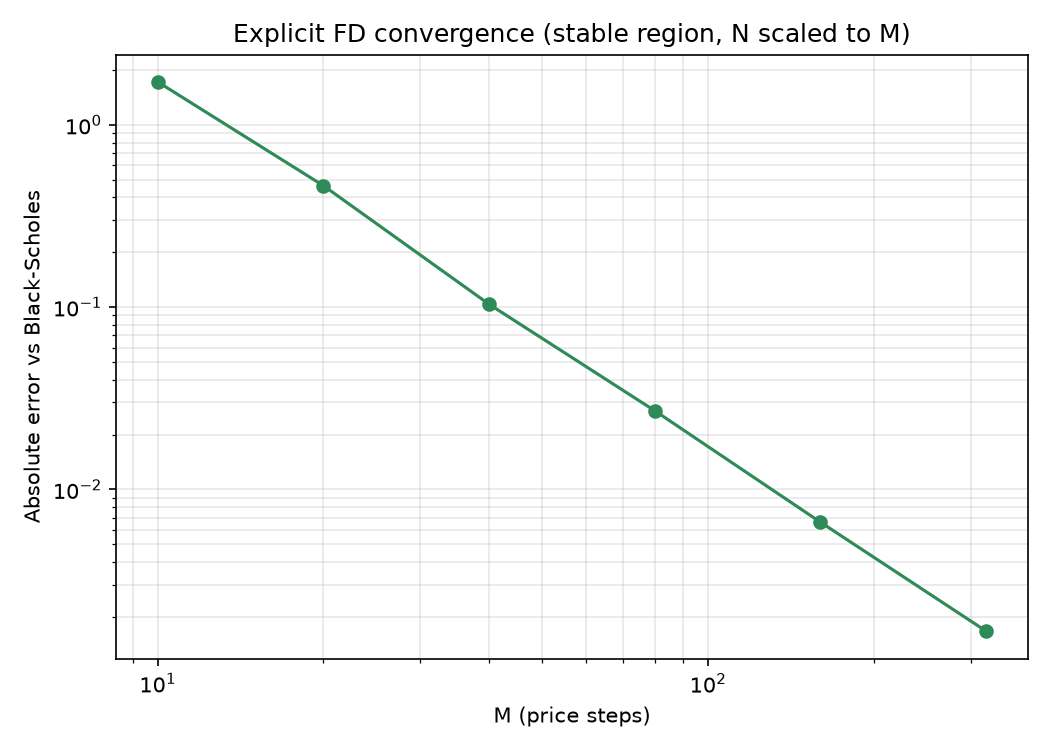
\includegraphics[width=0.92\textwidth]{pde_convergence.png}
  \caption{Error against the Black--Scholes price as the number of space steps
    $M$ increases, on log--log axes. The slope of $-2$ (the error quartering
    each time $M$ doubles) confirms second-order convergence in the space
    step.}
  \label{fig:pde-convergence}
\end{figure}

The method demonstrates the discretisation of a partial differential equation,
the conditional stability of the explicit scheme and how to diagnose it, and
second-order convergence measured against a known answer. It is this controlled
agreement that licenses applying the same machinery where no closed form exists.

% =====================================================================
\clearpage
\section{American options and early exercise}\label{sec:american}

An American option may be exercised at any time up to maturity, not only at $T$.
The holder must decide, at every moment, whether to exercise now or to hold; the
value is what an optimal exercise policy achieves. This is an optimal stopping
problem, and it has no closed-form solution even under the present model. The
binomial tree handles it with a single change.

\subsection{Early exercise in the tree}

At each node, compare the value of exercising immediately, the intrinsic value
$(K-S)^{+}$ for a put, with the value of holding, which is the discounted
risk-neutral expectation of the two child nodes. The node value is the larger of
the two,
\begin{equation}\label{eq:american}
  V = \max\Big(\, (K-S)^{+},\;
      e^{-r\Delta t}\big[\,p\,V_{\text{up}} + (1-p)\,V_{\text{down}}\,\big]\,\Big).
\end{equation}
The only difference from the European recursion \eqref{eq:crr-back} is the outer
maximum: one comparison at each node, asking whether exercising beats holding.
The nodes where exercise wins form the exercise region; elsewhere it is better to
hold. \Cref{fig:early-exercise} illustrates this for a put.

\begin{figure}[H]
  \centering
  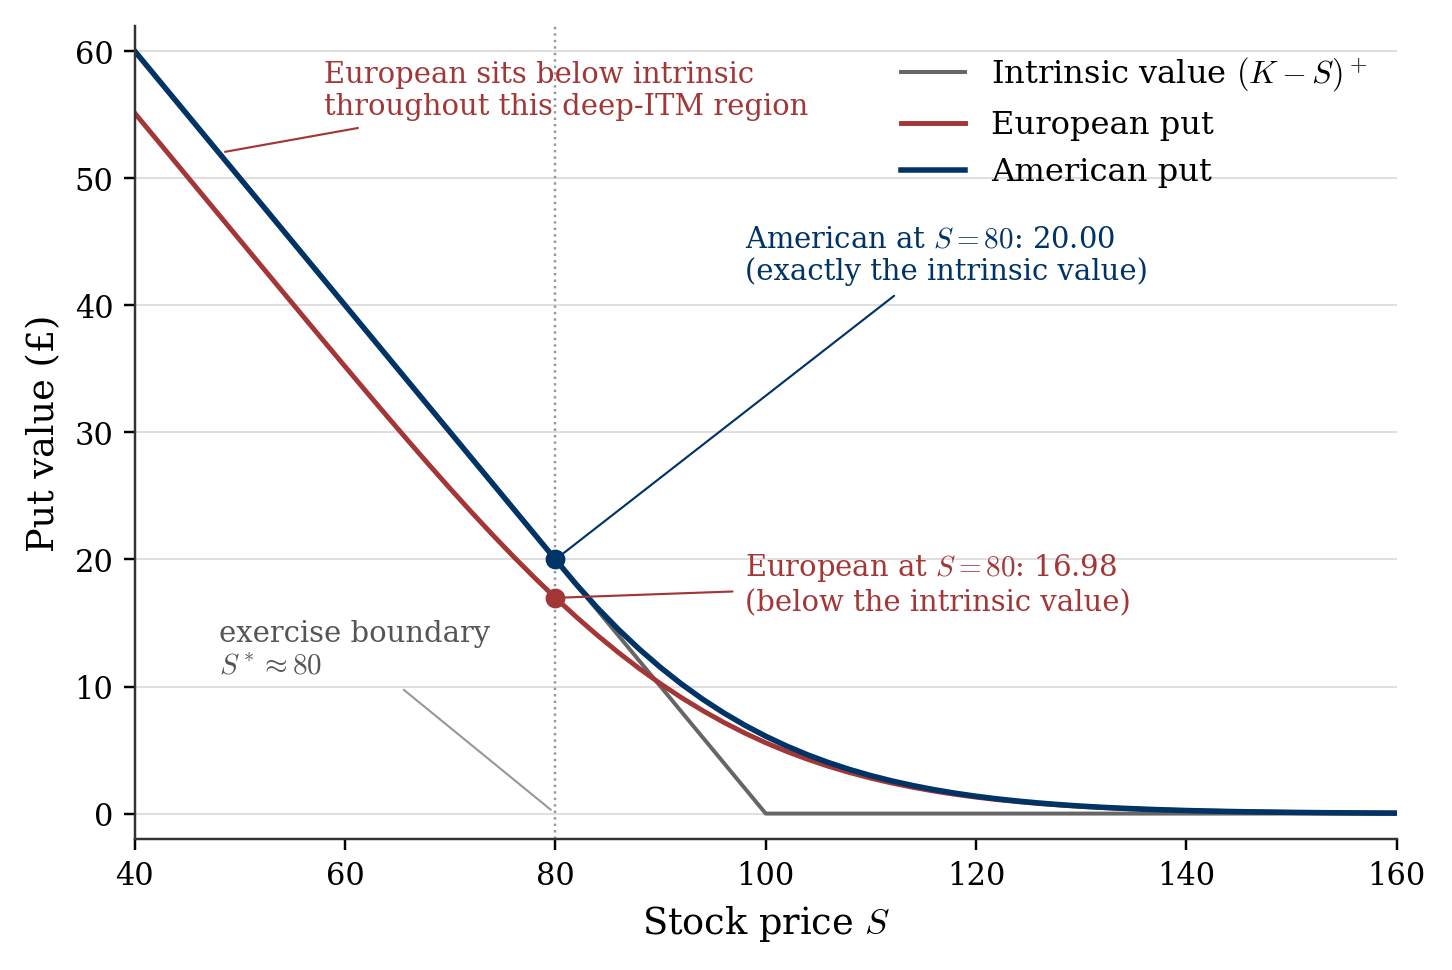
\includegraphics[width=0.92\textwidth]{american_comparison.png}
  \caption{Put value against the stock price, at the benchmark parameters
    ($K=100$, $r=5\%$, $\sigma=20\%$, $T=1$): the intrinsic value, the
    European put (Black--Scholes), and the American put (binomial tree,
    $N=400$). Below the exercise boundary $S^{\ast}$ the American value
    coincides exactly with the intrinsic value; the European value sits
    below the intrinsic value throughout the deep in-the-money region, since
    a European holder cannot realise that value until $T$.}
  \label{fig:early-exercise}
\end{figure}

\clearpage
\subsection{When early exercise matters}

A comparison against intrinsic value alone is not enough to show what is
distinctive about an American option. Both American and European options have
\emph{time value}: the chance that the stock moves favourably before $T$,
so both are generally worth more than today's cash-in value while time
remains; that is true of any option, not something special to the American
contract. The feature that is specific to the American option is the early
exercise \emph{right}, and the only way to see its effect is to compare the
American price against the European price for the same contract, which is
what \cref{fig:early-exercise} does.

Two features of that figure carry the argument. First, in the deep
in-the-money region the European curve sits \emph{below} the intrinsic
value: a European holder is locked in and must wait until $T$ to realise the
payoff, so today's value is a discounted, and therefore smaller, version of
it. Second, the American curve never does this: it cannot fall below
intrinsic value, because the holder always has the right to exercise
immediately and lock in that amount; arbitrage would otherwise be possible.
The gap between the navy and red curves in that region, vanishing above
$S^{\ast}$, is precisely the value of the early-exercise right, the
American-specific feature, isolated from ordinary time value.

It is worth being clear about what is being compared here in a different
sense too. Every method in
this report assumes no dividends throughout: that is a standing
simplification used everywhere, not something switched on or off in this
section. Given that, the comparison above is specific to puts. For a
call, by contrast, early exercise is never
optimal under this no-dividend assumption: holding is always worth at least the intrinsic value, because
exercising early forfeits both the interest earned by deferring payment of the
strike and the remaining time value. The American call therefore equals the
European call, with no early-exercise premium at all. (With dividends, a call
can sometimes be worth exercising just
before a payment, to capture it; that case does not arise here, since the
model has none.)

Both predictions are borne out numerically. For a deep in-the-money put at $S = 80$,
$K = 100$, the American price is exactly $20.0$, the intrinsic value $K - S$,
against a European put of $16.98$: an early-exercise premium of about $3.0$,
visible in \cref{fig:early-exercise} as the gap between the navy and red points
at $S=80$. For the call, the
American and European prices agree to eleven decimal places. The test suite checks
both: that the American put strictly exceeds the European put when deep in the
money, and that the American call equals the European call with no dividends.

The method demonstrates the early-exercise premium and the optimal-stopping
structure behind it. The tree accommodates early exercise almost for free, by the
single maximum in \eqref{eq:american}; the other two methods do not, for reasons
taken up next.

% =====================================================================
\clearpage
\section{Conclusion}\label{sec:conclusion}

The four methods price the benchmark European call in close agreement, as
\cref{tab:crossval} records. They differ by amounts consistent with their
respective numerical errors: the binomial and finite-difference values by small
discretisation errors, the Monte Carlo value by a sampling error of the size its
standard error predicts, which is evidence that the implementation is
correct.

\begin{table}[H]
  \centering
  \small
  \begin{tabular}{lcc}
    \toprule
    Method & Price & Difference from Black--Scholes \\
    \midrule
    Black--Scholes (closed form) & $10.4506$ & - \\
    Binomial tree (CRR, $N = 5000$) & $10.4502$ & $0.0004$ \\
    Monte Carlo ($10^{6}$ paths) & $10.4532 \pm 0.0147$ & $0.0026$ \\
    Explicit finite difference ($M = 200,\,N = 2000$) & $10.4550$ & $0.0044$ \\
    \bottomrule
  \end{tabular}
  \caption{The four methods at $S = K = 100$, $r = 5\%$, $\sigma = 20\%$,
    $T = 1$. The numerical methods agree with the exact price to within their
    expected errors.}
  \label{tab:crossval}
\end{table}

Each method also shows something the others do not. The closed form is exact and
fixes the reference. The binomial tree is a fully discrete scheme that converges
to the continuous price, with a visible odd--even oscillation along the way. Monte
Carlo is an unbiased estimator whose error is set by sample size and falls only as
$1/\sqrt{n}$, but which is indifferent to dimension. The finite-difference scheme
solves the governing equation directly and brings the sharpest numerical
questions with it: it is stable only when the time step is fine enough to keep the
central coefficient \eqref{eq:fd-coeffs} non-negative, and it converges at second
order in the space step, both confirmed here against the exact price. The American
extension adds the early-exercise premium and the optimal stopping that produces
it.

The scope was kept narrow on purpose, and the limitations follow from it.
Volatility and the interest rate are constant; the explicit scheme is only
conditionally stable; and the Monte Carlo and finite-difference treatments here
price European options. Three extensions follow naturally.

First, American pricing beyond the tree. In the tree early exercise is a single
comparison because each node carries its own continuation value. Monte Carlo does
not: a simulated path knows only its own future, not the continuation value at an
interior point, so that value must be estimated by regressing discounted future
payoffs on the current state, as in the Longstaff--Schwartz method
\cite{longstaffschwartz}. The finite-difference scheme must instead enforce the
exercise constraint at every grid point, which turns the equation into a linear
complementarity problem, solved by projected successive over-relaxation or a
penalty method.

Second, unconditional stability. The explicit scheme's condition \eqref{eq:cfl}
forces the number of time steps to grow with the square of the space refinement.
An implicit scheme, or the Crank--Nicolson scheme, is unconditionally stable and
removes that constraint, at the cost of solving a linear system at each step.

Third, beyond constant coefficients. Local or stochastic volatility, or a term
structure of interest rates, would be the next step towards a model that bears on
traded prices, and each of the methods developed here extends, with more work, to
accommodate it.

% =====================================================================
\clearpage
\begin{thebibliography}{9}
\bibitem{blackscholes} F.~Black and M.~Scholes,
  \emph{The pricing of options and corporate liabilities},
  Journal of Political Economy, 81(3):637--654, 1973.
  Available at \url{https://www.cs.princeton.edu/courses/archive/fall09/cos323/papers/black_scholes73.pdf}.
\bibitem{crr} J.~C. Cox, S.~A. Ross and M.~Rubinstein,
  \emph{Option pricing: a simplified approach},
  Journal of Financial Economics, 7(3):229--263, 1979.
\bibitem{longstaffschwartz} F.~A. Longstaff and E.~S. Schwartz,
  \emph{Valuing American options by simulation: a simple least-squares approach},
  Review of Financial Studies, 14(1):113--147, 2001.
  Available at \url{http://galton.uchicago.edu/~mykland/346W07/Longstaff.pdf}.
\bibitem{ammari} H.~Ammari,
  \emph{Numerical Methods for ODEs, Lecture 6: Finite difference methods},
  Department of Mathematics, ETH Z\"urich.
  Available at \url{https://people.math.ethz.ch/~grsam/SS23/NAII/resources/slides/ODE-Lecture6.pdf}.
\end{thebibliography}

\vspace{1em}
\noindent\textbf{Further reading.} Readers seeking a fuller, textbook-length
treatment of this material may consult the standard references: P.~Wilmott,
\emph{Paul Wilmott on Quantitative Finance}, 2nd edition, Wiley, 2006;
P.~Glasserman, \emph{Monte Carlo Methods in Financial Engineering}, Springer,
2003; and D.~J. Higham, \emph{An Introduction to Financial Option Valuation},
Cambridge University Press, 2004.

\end{document}